\documentclass{article}
\usepackage[utf8]{inputenc}
\usepackage{graphicx}
\usepackage[a4paper,
            left=1in,
            right=1in,
            ]{geometry}
\usepackage{float}
\usepackage[table,xcdraw]{xcolor}

\author{Dawid Stasiak}
\title{Report}

\begin{document}

\maketitle

\tableofcontents
\newpage

\setlength\parindent{0pt}

This is the documentation regarding the project. I will discuss here
how I analysed the data, I will give here any findings that I find
relevant to the task, the choices and assumptions I have made, and
results.

\section{Data Description}

In this section I would like to present the findings of the performed
data analysis, this will allow me to make informed choices regarding
data cleaning and any assumptions and methods used.

\subsection{Text Data - Number of Facts}

In the following plot we display the box plots showing the number of
facts for each case in each dataset (train, test and validation).

\begin{figure}[H]
    \centering
    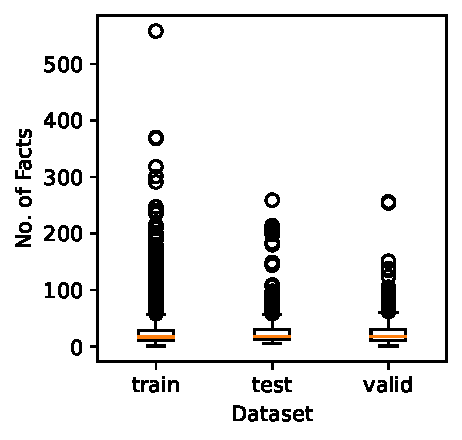
\includegraphics[scale=0.8]{facts_boxplots.pdf}
    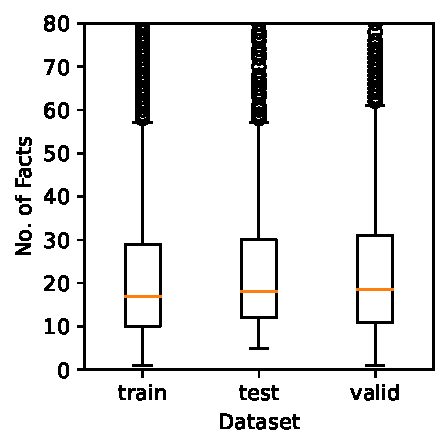
\includegraphics[scale=0.8]{facts_boxplots_cutoff.pdf}
    \caption{Box plots detailing the number of facts for each case and
    each dataset, each point represents a single case. Plot on the
    left shows all cases, and plot on the right has been cut off to
    zoom in on the averages.}
    \label{fig: facts box plots}
\end{figure}

We can see that all sets have a similar average number of facts, we
can conclude that the datasets are well balanced with regard to the
number of facts per case.
\begin{table}[H]
\centering
\begin{tabular}{|l|c|c|c|}
\hline
\rowcolor[HTML]{C0C0C0} 
\multicolumn{1}{|c|}{\cellcolor[HTML]{C0C0C0}statistic} & train & test & validation \\ \hline
min & 1 & 5 & 1 \\
max & 558 & 259 & 256 \\
mean & 23.65 & 25.28 & 24.41 \\
median & 17 & 18 & 18.5 \\ \hline
\end{tabular}
\caption{Extracted statistics regarding the number of facts per case for each dataset.}
\label{tab: facts per case statistics}
\end{table}

\subsection{Label Data}

Each dataset (train, test and validation) have the same set of unique
labels, the unique articles for all datasets range from 
0 to 9 (there are 10 different possible articles that can be violated) and
each dataset uses all of them.

\begin{table}[H]
\centering
\begin{tabular}{l|c}
Dataset    & Articles/Case \\ \hline
train      & 1.18          \\
test       & 1.09          \\
validation & 1.06         
\end{tabular}
\caption{Number of violated articles per case for each dataset}
\label{tab: articles per case}
\end{table}

In the next plot we want to show the proportion of labels in each 
dataset and see how they compare.

\begin{figure}[H]
    \centering
    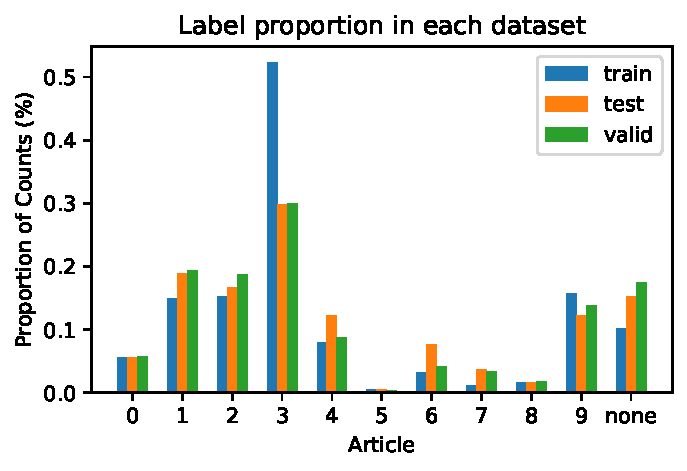
\includegraphics[]{label_proportions.pdf}
    \caption{Proportion of Articles in each dataset}
    \label{fig: label proportions}
\end{figure}

We can see that article number 5 has been violated least amounts of times and
article number 3 the most amount of times in each dataset.
The datasets are not very well balanced, i.e. there are articles which
are violated more often than others. In a well balanced dataset each
article would have an equal representation, this is not the case in our
dataset as seen in the bar chart above.

\section{Method}

In this section I would like to state the methods I have used 
to classify the court cases.\\

I have chosen to work on the ecthr\_a dataset. The dataset
contains court case facts as features in text-form and attached
to the court cases are labels which state which articles have
been violated in the court case. The goal of this task is to train
a machine learning model to predict the violated articles given the 
records of a court case. The training examples contain
both the text and labels (therefore supervised learning can be used).\\

The task is split into two steps:

\begin{enumerate}
    \item The text-data needs to be
        transformed into a datatype that can be read by a neural network.
        This will be done by sentence embedding. 
        A method of representing sentences as numerical vectors of 
        task-specific dimensions. In this work, the dimension of the 
        embedding space will be $512$. This dimension has been chosen due to 
        the limitation of the model used. There exist pretrained models
        that are capable of embedding sentences into vectors. I have
        used an already pre-trained model for embedding the text-data in
        this work. The model used is a transformer-based model
        based on Bidirectional Transformers for Language Understanding 
        \cite{DBLP:journals/corr/abs-1810-04805}
        or BERT for short. Embedding consists of tokenizing the sentences
        where I joined all the facts of a case into one large sentence
        and tokenized the sentence using BertTokenizerFast 
        \cite{DBLP:journals/corr/abs-1810-04805} found in the 
        transformers Python library. The tokenizer is only able to encode
        up to 512 tokens. This a limitation of the model and can lead
        to compromised results as we cannot use all the text data available
        to us as we are working with large documents, which
        more often than not contain 512 words. The reason we use this
        model is because it has been shown to give best results in a 
        very similar task \cite{DBLP:journals/corr/abs-1906-02059}, 
        despite this limitation.

    \item The second step in this pipeline is, once we have embedded our
        sentences into a vector space, we can train a neural network
        to predict the broken articles for each case using the generated 
        embeddings. 
        There are many ways again to use the embeddings for multi-class
        classification. There exist many models capable of multi-class
        classification, and different ways of approaching the task based
        on assumptions made. My assumption was that the labels
        are not independent of each-other, i.e. that if one article is 
        violated, perhaps another article is likely to be violated too.
        I have not had time to check if this assumption is true, but it
        is an assumption I have made 
        by using the BertModel \cite{DBLP:journals/corr/abs-1810-04805} 
        found in the transformers library in Python.
        Another way of approaching a multi-classification task would
        be to treat each article to be independently violated, i.e.
        if one article is violated it has no effect on other articles
        being violated. In this case you could build many smaller
        classifiers which would each predict a single article to
        be violated or not. This is not the approach I have taken here.
        I chose to use the method I have used as it showed the best results
        in a similar task \cite{DBLP:journals/corr/abs-1906-02059}, 
        compared to the many-models approach.
\end{enumerate}

For training the model, I have used the pytorch\_lightning library.
Which is a library I wanted to try and use for some time.
It automates many of the training steps such as passing the model
and the data to the gpu, it monitors the training and saves
a model checkpoint automatically based on some conditions, can be used
to load the saved model checkpoint etc.
\\

I have modified the BertModel slightly by building on top of it
a linear layer that takes in the output of the BertModel and returns
a vector of size 10 followed by a sigmoid function. The output of the linear
layer is
10 dimensional corresponding to the 10 different articles that can
be violated. Each value in the output can range from 0 to 1 and
will be treated as the chance of that article being broken, with
the threshold being 0.5.
The labels are converted to 10 dimensional vectors too, to 
match the output of the neural network. Thus we are building a
binary multi-class classifier. The labels are k-hot vectors.\\

The loss function used is the Binary Cross Entropy Loss (BCELoss),
that is capable of obtaining a loss in multi-class scenarios.\\

I only ran a single training session as training for 10 epochs takes
roughly 3 hours. I used the entire training dataset containing 9000
training examples to train the model, with a learning rate
of 2e-5. 
The training ran for 2 epochs before being stopped
early by pytorch\_lightning training module, which has detected that
the loss has not been going down further, deciding to stop the
training. The patience of the early stop can be modified.\\

The trained model was saved to a checkpoint which can be loaded.
The trained model takes up 1.3GB of storage and is thus not 
provided in the github repository. \\

We can use the saved model and pass through it the unseen validation
or test set, to see how the model performs on unseen data.
I pass the validation and test set through the trained model
generating predictions. I save the predictions using the pickle
library, so that I have easy access to them.
I calculate the precision, recall and f1-score for each article 
individually, see next section for results. Then I compute the 
micro, macro, weighted and sample averages for all articles
in both the validation and test datasets.
The reason for those metrics is the imbalanced nature of our datasets
not every article has an equal representation, and this needs to
be accounted for. Precision, recall and the f1-score are good
metrics when working with imbalanced data.


\section{Results}

\begin{table}[H]
    \centering
    \begin{tabular}{|l|c|c|c|c|}
    \hline
        Article & Precision & Recall & F1-Score & Support \\ \hline
        0 & 0.82 & 0.66 & 0.73 & 56 \\ \hline
        1 & 0.65 & 0.75 & 0.70 & 189 \\ \hline
        2 & 0.79 & 0.51 & 0.62 & 166 \\ \hline
        3 & 0.70 & 0.57& 0.63& 299 \\ \hline
        4 & 0.70& 0.31& 0.43& 123 \\ \hline
        5 & 0.0 & 0.0 & 0.0 & 5 \\ \hline
        6 & 0.61& 0.40& 0.48& 77 \\ \hline
        7 & 0.82& 0.24& 0.37& 37 \\ \hline
        8 & 0.0 & 0.0 & 0.0 & 16 \\ \hline
        9 & 0.70& 0.79& 0.73& 122 \\ \hline
        Micro Avg & 0.70& 0.56& 0.62& 1090 \\ \hline
        Macro Avg & 0.58& 0.42& 0.47& 1090 \\ \hline
        Weighted Avg & 0.70& 0.56& 0.60& 1090 \\ \hline
        Samples Avg & 0.53& 0.49& 0.50& 1090 \\ \hline
    \end{tabular}
    \caption{Model results on test dataset. I calculate Precision, 
    Recall and F1-Score individually for each article label. 
    Test set contains 1000 examples.
    Support is the number of true positives for that article}
\end{table}

\begin{table}[H]
    \centering
    \begin{tabular}{|l|c|c|c|c|}
    \hline
        Article & Precision & Recall & F1-Score & Support \\ \hline
        0 & 0.78 & 0.63 & 0.70 & 57 \\ \hline
        1 & 0.69 & 0.69 & 0.69 & 193 \\ \hline
        2 & 0.80 & 0.54 & 0.65 & 187 \\ \hline
        3 & 0.71 & 0.6 & 0.65 & 300 \\ \hline
        4 & 0.49 & 0.25 & 0.33 & 87 \\ \hline
        5 & 0.0 & 0.0 & 0.0 & 4 \\ \hline
        6 & 0.67 & 0.67 & 0.67 & 42 \\ \hline
        7 & 1.0 & 0.36 & 0.53 & 33 \\ \hline
        8 & 0.5 & 0.06 & 0.10 & 18 \\ \hline
        9 & 0.72 & 0.81 & 0.76 & 139 \\ \hline
        Micro Avg & 0.71 & 0.59 & 0.65 & 1060 \\ \hline
        Macro Avg & 0.64 & 0.46 & 0.51 & 1060 \\ \hline
        Weighted Avg & 0.71 & 0.59 & 0.63 & 1060 \\ \hline
        Samples Avg & 0.54 & 0.51 & 0.51 & 1060 \\ \hline
    \end{tabular}
    \caption{Model results as above but for the validation dataset. 
    Validations dataset contains 1000 examples.}
\end{table}

\newpage

\bibliography{refs}
\bibliographystyle{ieeetr}
    
\end{document}
